%ne rien compléter dans le main! ;)

\documentclass[11pt,a4paper]{article}
\usepackage[top=1in, bottom=1in, left=1in, right=1in]{geometry}

%%%%%%%%%%%%%%%%
%%% PACKAGES %%%
%%%%%%%%%%%%%%%%

\usepackage{ucs}
\usepackage[T1]{fontenc}
\usepackage{amsmath}
\usepackage{amsthm}
\usepackage{dsfont}
\usepackage{amsfonts}
\usepackage{amssymb}
\usepackage{mathtools}
\usepackage[utf8]{inputenc} 
%\usepackage[french]{babel}
\usepackage[framemethod=tikz]{mdframed}

%packages spéciaux
\usepackage{fullpage}
\usepackage{mathrsfs}
\usepackage{numprint}
\usepackage{graphicx}
\usepackage{hyperref}
\usepackage{float}

\usepackage[numbered,framed,autolinebreaks]{misc/mcode}
\usepackage{sfmath}
\usepackage{sansmathaccent}
\usepackage{cmbright}

\usepackage{misc/slashbox}
\usepackage{placeins} % permet d'utiliser \FloatBarrier et donc d'imposer le placement des images dans une section donnée.
\usepackage{multirow}

\newcommand\scalemath[2]{\scalebox{#1}{\mbox{\ensuremath{\displaystyle #2}}}}
\newcommand{\HRule}{\rule{\linewidth}{0.5mm}}



%%%%%%%%%%%%%
%%% INFOS %%%
%%%%%%%%%%%%%

\title{System Identification and Modeling - Part I}
\author{Willem Melis (r0348639) and Marie Valenduc (r0656511)}
\date{\today}

%%%%%%%%%%%%%%%%
%%% DOCUMENT %%%
%%%%%%%%%%%%%%%%

\begin{document}

%NE PAS TOUCHER A CETTE PAGE
\begin{titlepage}
\begin{center}

%\includegraphics[width=18cm]{Figures/KUL-LOGO.png}~\\[1cm]
\vfill


\textsc{\LARGE Katholieke Universiteit Leuven}\\[0.7cm]

\textsc{\Large System Identification and Modeling}\\[0.7cm]

% titre
\begin{mdframed}[backgroundcolor=none,fontcolor=black,innerbottommargin=0.7cm, innertopmargin=0.6cm, linewidth=2pt]
    \centering \huge \bfseries Exercises - Part 1 
\end{mdframed}

\end{center}

\vfill

% auteurs et tuteur
\begin{center}
\emph{Authors:} \\[.2cm]
\begin{tabular}[h]{rl}
Marie \textsc{Valenduc} & r0656511\\
Willem \textsc{Melis} & r0348639\\
\phantom{------------------------} & \phantom{------------------------}\\
\end{tabular}
\end{center}

\vfill

\begin{center}
\begin{tabular}[h]{rl}
\emph{Professor:} & Philippe \textsc{Dreesen}\\
\emph{Assistants:}&  Olivier \textsc{Lauwers} \\
&  Bob \textsc{Vergauwen} \\
\phantom{------------------------} & \phantom{------------------------}\\
\end{tabular}
\end{center}

\vfill
\vfill
\vfill

%date
\begin{center} 
2016 - 2017 \\[.5cm]
{\Large \today}
\end{center}

\end{titlepage}

%\tableofcontents 
\part{Noise on Input and Output.}
In order to calculate the asymptotic value of the estimates, we will use the following statistical tools:
\begin{itemize}
    \item $\lim\limits_{N \rightarrow +\infty} \frac{1}{N} \sum_{k=0}^N x(k) = \mu_x $
    \item $\lim\limits_{N \rightarrow +\infty} \frac{1}{N} \sum_{k=0}^N (x(k) - \mu_x)^2 = \sigma_x^2 $
    \item For the mutually uncorrelated signals $x(k)$ and $y(k)$ holds $\lim\limits_{N \rightarrow +\infty} \frac{1}{N} \sum_{k=0}^N x(k) y(k) = 0 $
\end{itemize}

Using the facts that $\mu_{n_i}$ = $\mu_{n_u}$ $\mu_{i_0}$ = 0 and $i_0$, $n_i$ and $n_u$ are independent, we obtain: 

\begin{equation}\label{as_val_LS}
    \lim\limits_{N \rightarrow +\infty} \hat{R}_{LS} = R_0 \frac{1}{1+\frac{\sigma_{n_i}^2}{\sigma_{i_0}^2}}
\end{equation}

\begin{equation}\label{as_val_IV}
        \lim\limits_{N \rightarrow +\infty} \hat{R}_{IV} = R_0 \frac{1}{1+\frac{R_{n_i n_i}(s)}{R_{i_0 i_0}(s)}}
\end{equation}
where $R_{x x}(l) = \lim\limits_{N \rightarrow +\infty} \frac{1}{N} \sum_{k=1}^N x(k) x(k-l)$ is the autocorrelation function of $x$.

\section{Experiment 1 : influence of the filtering of the input noise.}
For the first experiment, we use the following parameter settings : 

\begin{table}[h]
\centering
\begin{tabular}{lll}
    $ R_0 = 1000, $  &  $ f_{gen} = 0.1, $ & $ f_{noise} = \{ 0.999, 0.95, 0.6 \},$  \\
    $ \sigma_{i_0} = 0.1, $  &  $ \sigma_{n_i} = 0.1, $ & $ \sigma_{n_u} = 1.$  \\
\end{tabular}
\end{table}
The result of the first experiment are displayed on the figure~\ref{Sess1_part1_exp1}.

\paragraph{LS estimate} As can be seen on the top picture of fig.~\ref{Sess1_part1_exp1}, the LS estimate is strongly biased. This can be explained by using Eq. \ref{as_val_LS}: the  relative bias is in the order of $\frac{\sigma_{n_i}^2}{\sigma_{i_0}^2}$. With the above parameter settings, we obtain the following asymptotic value :
$$ \lim\limits_{N \rightarrow +\infty} \hat{R}_{LS} = R_0 \frac{1}{2}  = 500 $$ 
The values of the LS estimate are indeed always around 500. This bias is due to the fact that, with the LS estimate, we assume that the measured input is exact, which is not the case here because of the noise $n_i$. 

\paragraph{IV estimate} Considering Eq.~\ref{as_val_IV}, we conclude that the smaller is the ratio $\frac{R_{n_i n_i}(s)}{R_{i_0 i_0}(s)}$, the less biased is the IV estimate. 
Here, the input noise $n_i$ is generated by filtering a white noise $e_2$ by a second order Butterworth filter of parameter $f_{noise}$. 

We analyse the asymptotic value of $\hat{R}_{IV}$ in function of the parameter $f_{noise}$. Since $R_{i_0 i_0}(s)$ is kept constant, we will only talk about $R_{n_i n_i}(s)$.
\begin{itemize}
    \item if $f_{noise} = 0.999$, the generated input noise $n_i$ is a white noise. The auto-correlation function $R_{n_i,n_i}(s)$ exhibits a peak in $s = 0$ and is then absolutely 0 for all other $s$. Therefore, $R_{n_i,n_i}(1) = 0$ and the IV estimate for $s = 1$ converges to $R_0$. There is thus no bias present. On fig.~\ref{Sess1_part1_exp1} (a), we see that the mean value of IV(1) is close to $R_0$.
    \item if $f_{noise} = 0.9$, the IV estimate will have a small bias : indeed, we notice on fig.~\ref{Sess1_part1_exp1} (b.2) that the auto-correlation function $R_{n_i,n_i}(s)$ is not perfectly equal (but close) to 0 at $s=1$. The mean value IV(2) on fig.~\ref{Sess1_part1_exp1} (a) is 938 and is thus close to the searched value.
    \item if $f_{noise} = 0.6$, the bias will be bigger; $R_{n_i,n_i}(1)$ is indeed larger than in the two other cases. The mean value IV(3) on fig.~\ref{Sess1_part1_exp1} (a) is 645 and is thus far from $R_0$.
\end{itemize}

As a conclusion, the results are strongly influenced by the filter : the larger $R_{n_i,n_i}(s)$, the larger the bias will be.
\begin{figure}[h!]
    \centering
    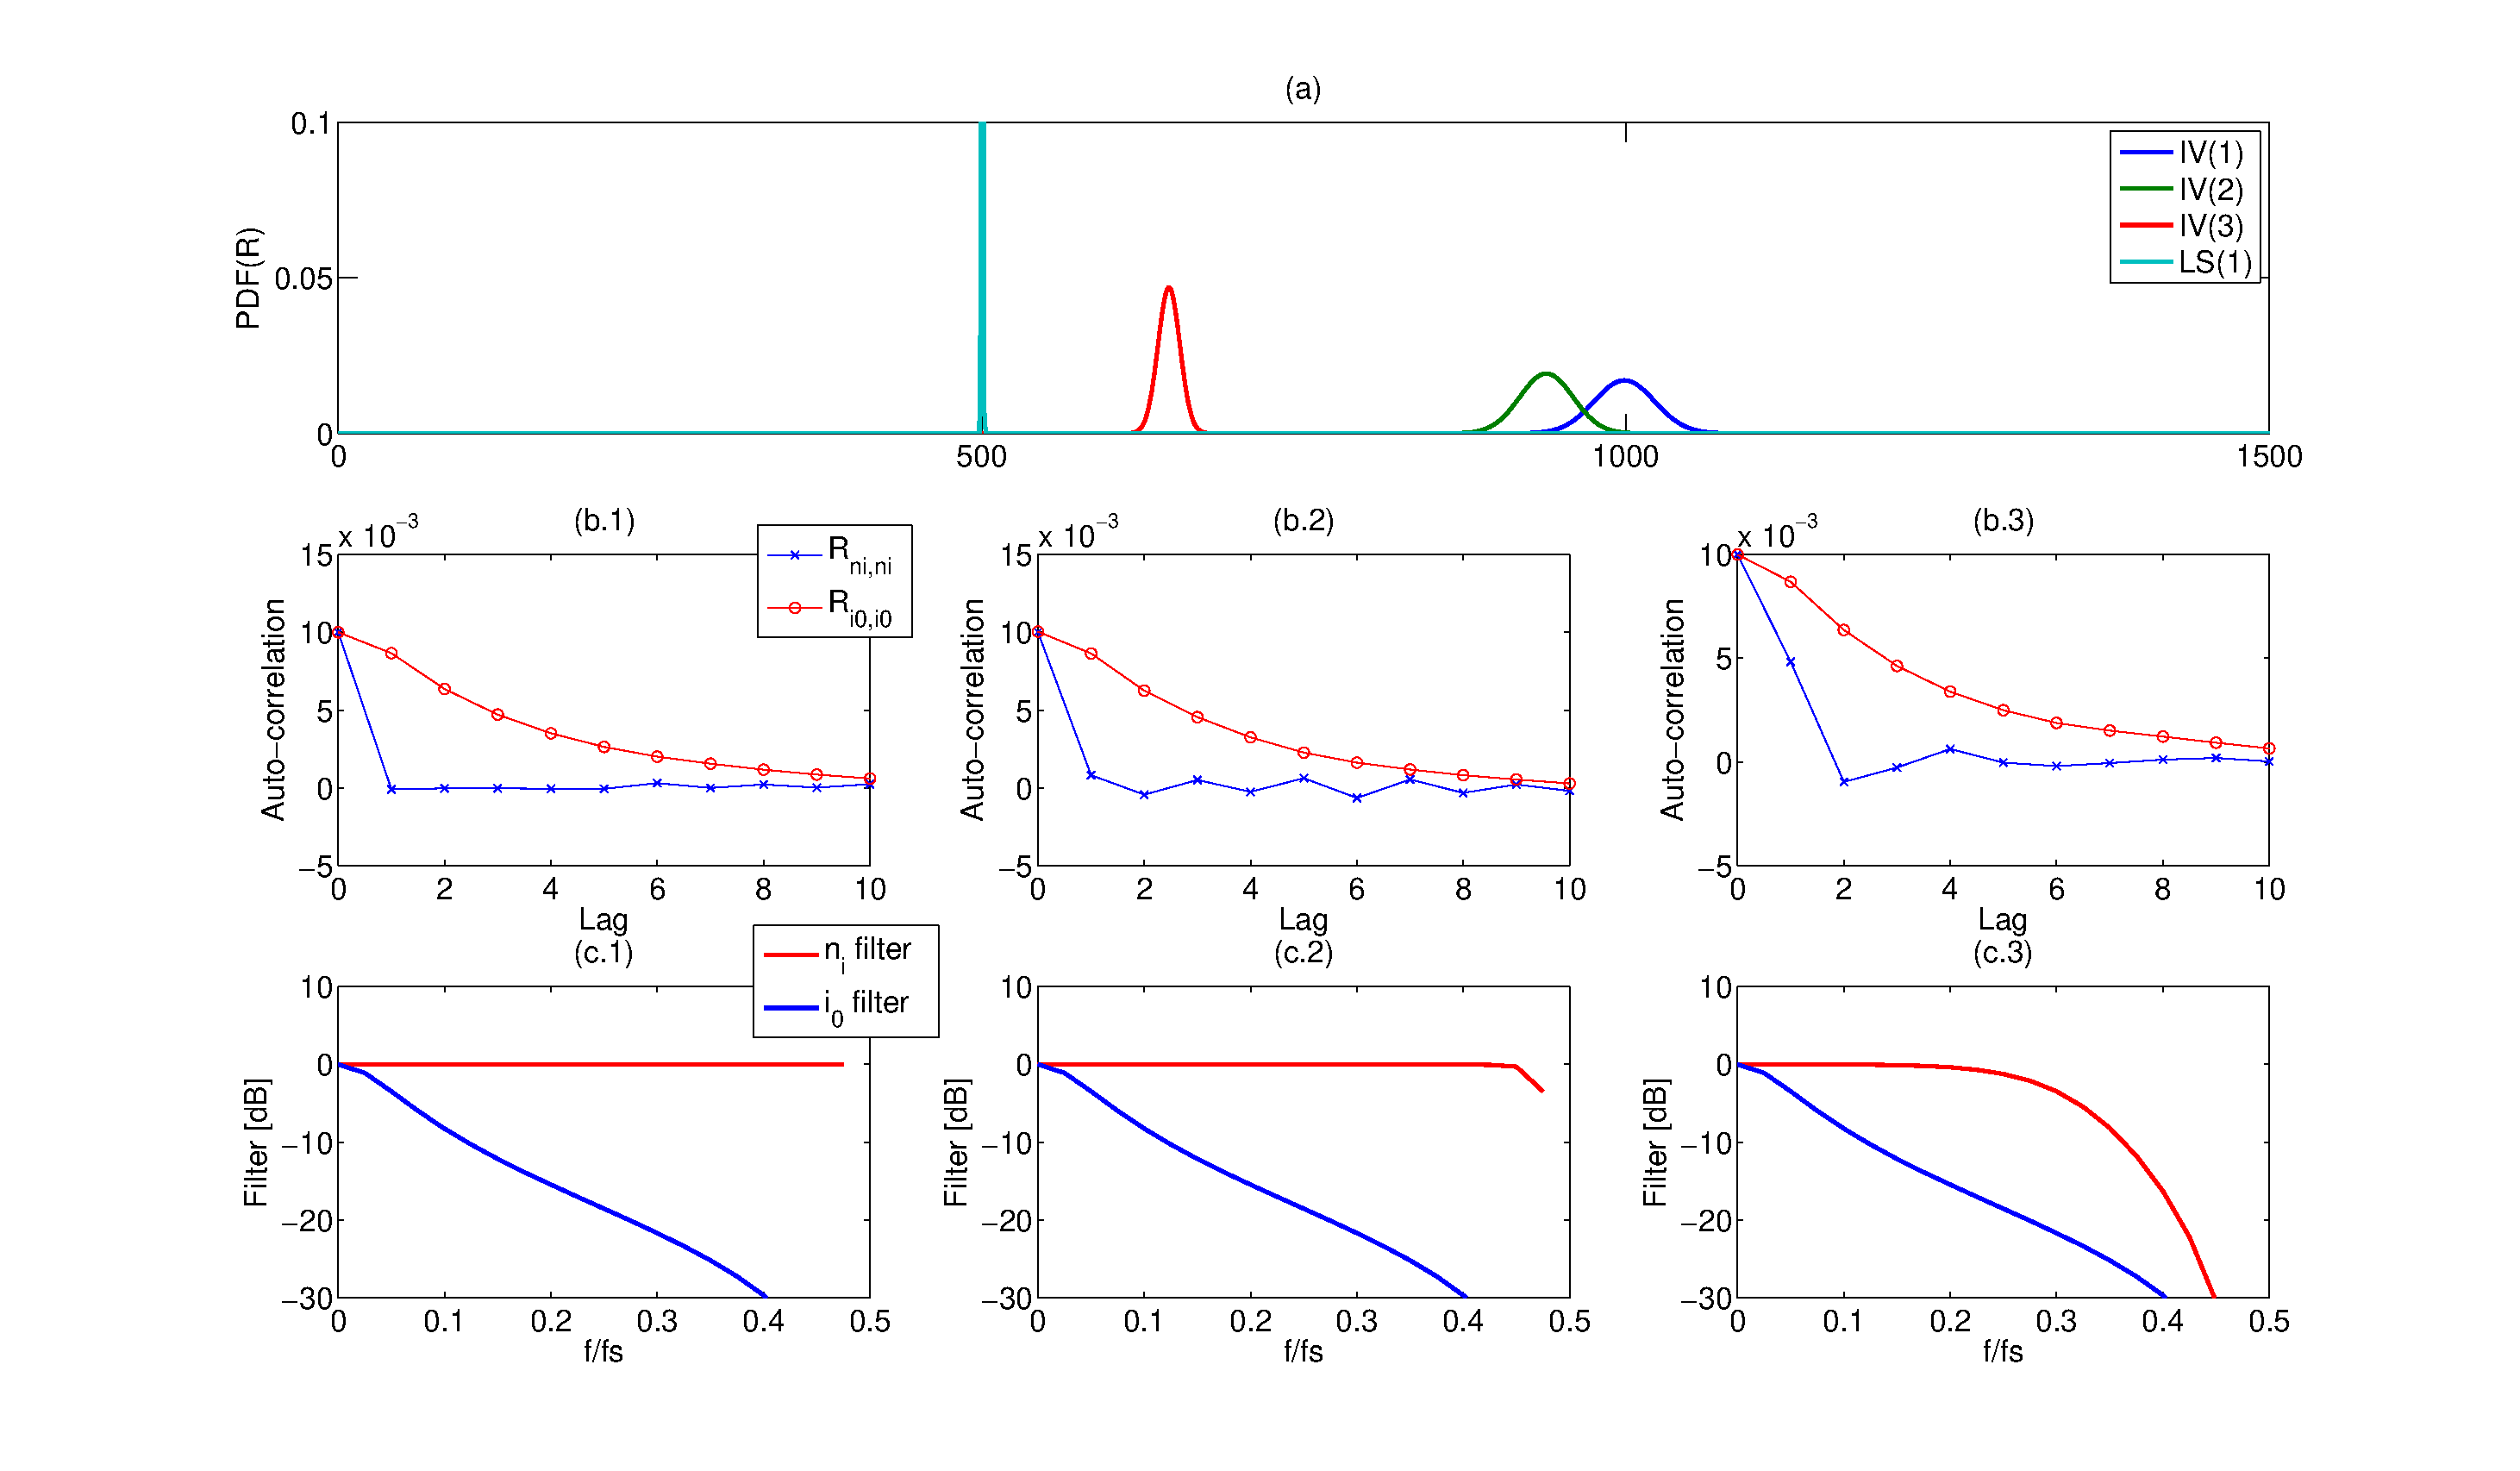
\includegraphics[width=1\textwidth]{Figures/Sess1_part1_exp1.eps}
    \caption{Study of the LS and IV estimates for a varying noise filter bandwidth and fixed shift parameter $s = 1$. Fig.~(a) : the LS (cyan) and IV estimates. IV(1) (blue), IV(2) (green) and IV(3) (red) correspond to the noise filters with cut-off frequencies 0.999, 0.95 and 0.6 respectively. Fig.~(b) : the auto-correlation of $i_0$ (red) and $n_i$ (blue) for the different noise filters. Fig.~(c): filter characteristics of $i_0$ (blue) and of $n_i$ (red).}
    \label{Sess1_part1_exp1}
\end{figure}


\section{Experiment 2 : influence of the parameter s.}
For the second experiment, we use the following parameter settings : 
\begin{table}[h]
\centering
\begin{tabular}{lll}
    $ R_0 = 1000, $  &  $ f_{gen} = 0.1, $ & $ f_{noise} = 0.6 ,$  \\
    $ \sigma_{i_0} = 0.1, $  &  $ \sigma_{n_i} = 0.1, $ & $ \sigma_{n_u} = 1.$  \\
\end{tabular}
\end{table}

The purpose here is to analyze the influence of the shift $s$ on the estimation by making it vary ($s = 1, 2$ and $5$) with constant filters. The results are displayed on figure \ref{fig: Sess1_part1_exp2}. Moreover, the most important results are visible in table \ref{tab: Sess1_part1_exp2}. 

As we increase the shift $s$, we can see that $\hat{R}_{IV}$ becomes closer to the searched value $R_0 = 1000$, i.e. the bias becomes smaller. This is because the ratio $R_{n_i n_i}(s)/R_{i_0 i_0}(s)$ becomes smaller with increasing $s$ (cfr. table \ref{tab: Sess1_part1_exp2}). We observe that the sign of the bias depends on the sign of $R_{n_i n_i}(s)$. This can be seen by looking at equation~\ref{as_val_IV} : if $R_{n_i n_i}(s) \ge 0$, the factor $(1+R_{n_i n_i}(s)/R_{i_0 i_0}(s))^{-1}$ is smaller than 1, which results in an under-estimation of $R_0$. At the other hand, if $R_{n_i n_i}(s) \le 0$, a similar reasoning leads to the conclusion that $R_0$ will be over-estimated. That is indeed what we observe in table~\ref{tab: Sess1_part1_exp2}.

\begin{table}[ht]
\centering
\begin{tabular}{|c|c|c|c|c|c|}
\hline
$s$ & $R_{n_i n_i}(s)$ & $R_{i_0 i_0}(s)$ & $R_{n_i n_i}(s)/R_{i_0 i_0}(s)$ & theoretical $\hat{R}_{IV}$ & experimental $\hat{R}_{IV}$ \\
\hline
\hline
1 & 0.0048 & 0.0086 & 0.5532 & 634 & $\mu$ = 645.44\\
\hline
2 & -0.0012 & 0.0062 & -0.1953 & 1242 & $\mu$ = 1226.5 \\
\hline
5 & -0.0001 & 0.0021 & -0.0435 & 1045 & $\mu$ = 1039.33 \\
\hline
\end{tabular}\caption{}\label{tab: Sess1_part1_exp2}
\end{table}
However, the IV estimates does not seem to be the perfect choice since its variance keeps increasing with $s$. This is mainly due to the auto-correlation function of the current $R_{i_0 i_0}(s)$  that becomes smaller with increasing shift $s$. We can compute an approximation of the variance by neglecting the second order terms and by doing a Taylor series expansion. This leads to :
\begin{equation}
\lim\limits_{N \rightarrow +\infty} \sigma^2_{\hat{R}_{IV}} = \sigma^2_{n_u} \frac{\sigma^2_{n_i}  + \sigma^2_{i_0}}{(R_{n_i n_i}(s) + R_{i_0 i_0}(s))^2}
\end{equation}


\begin{figure}[H]
    \centering
    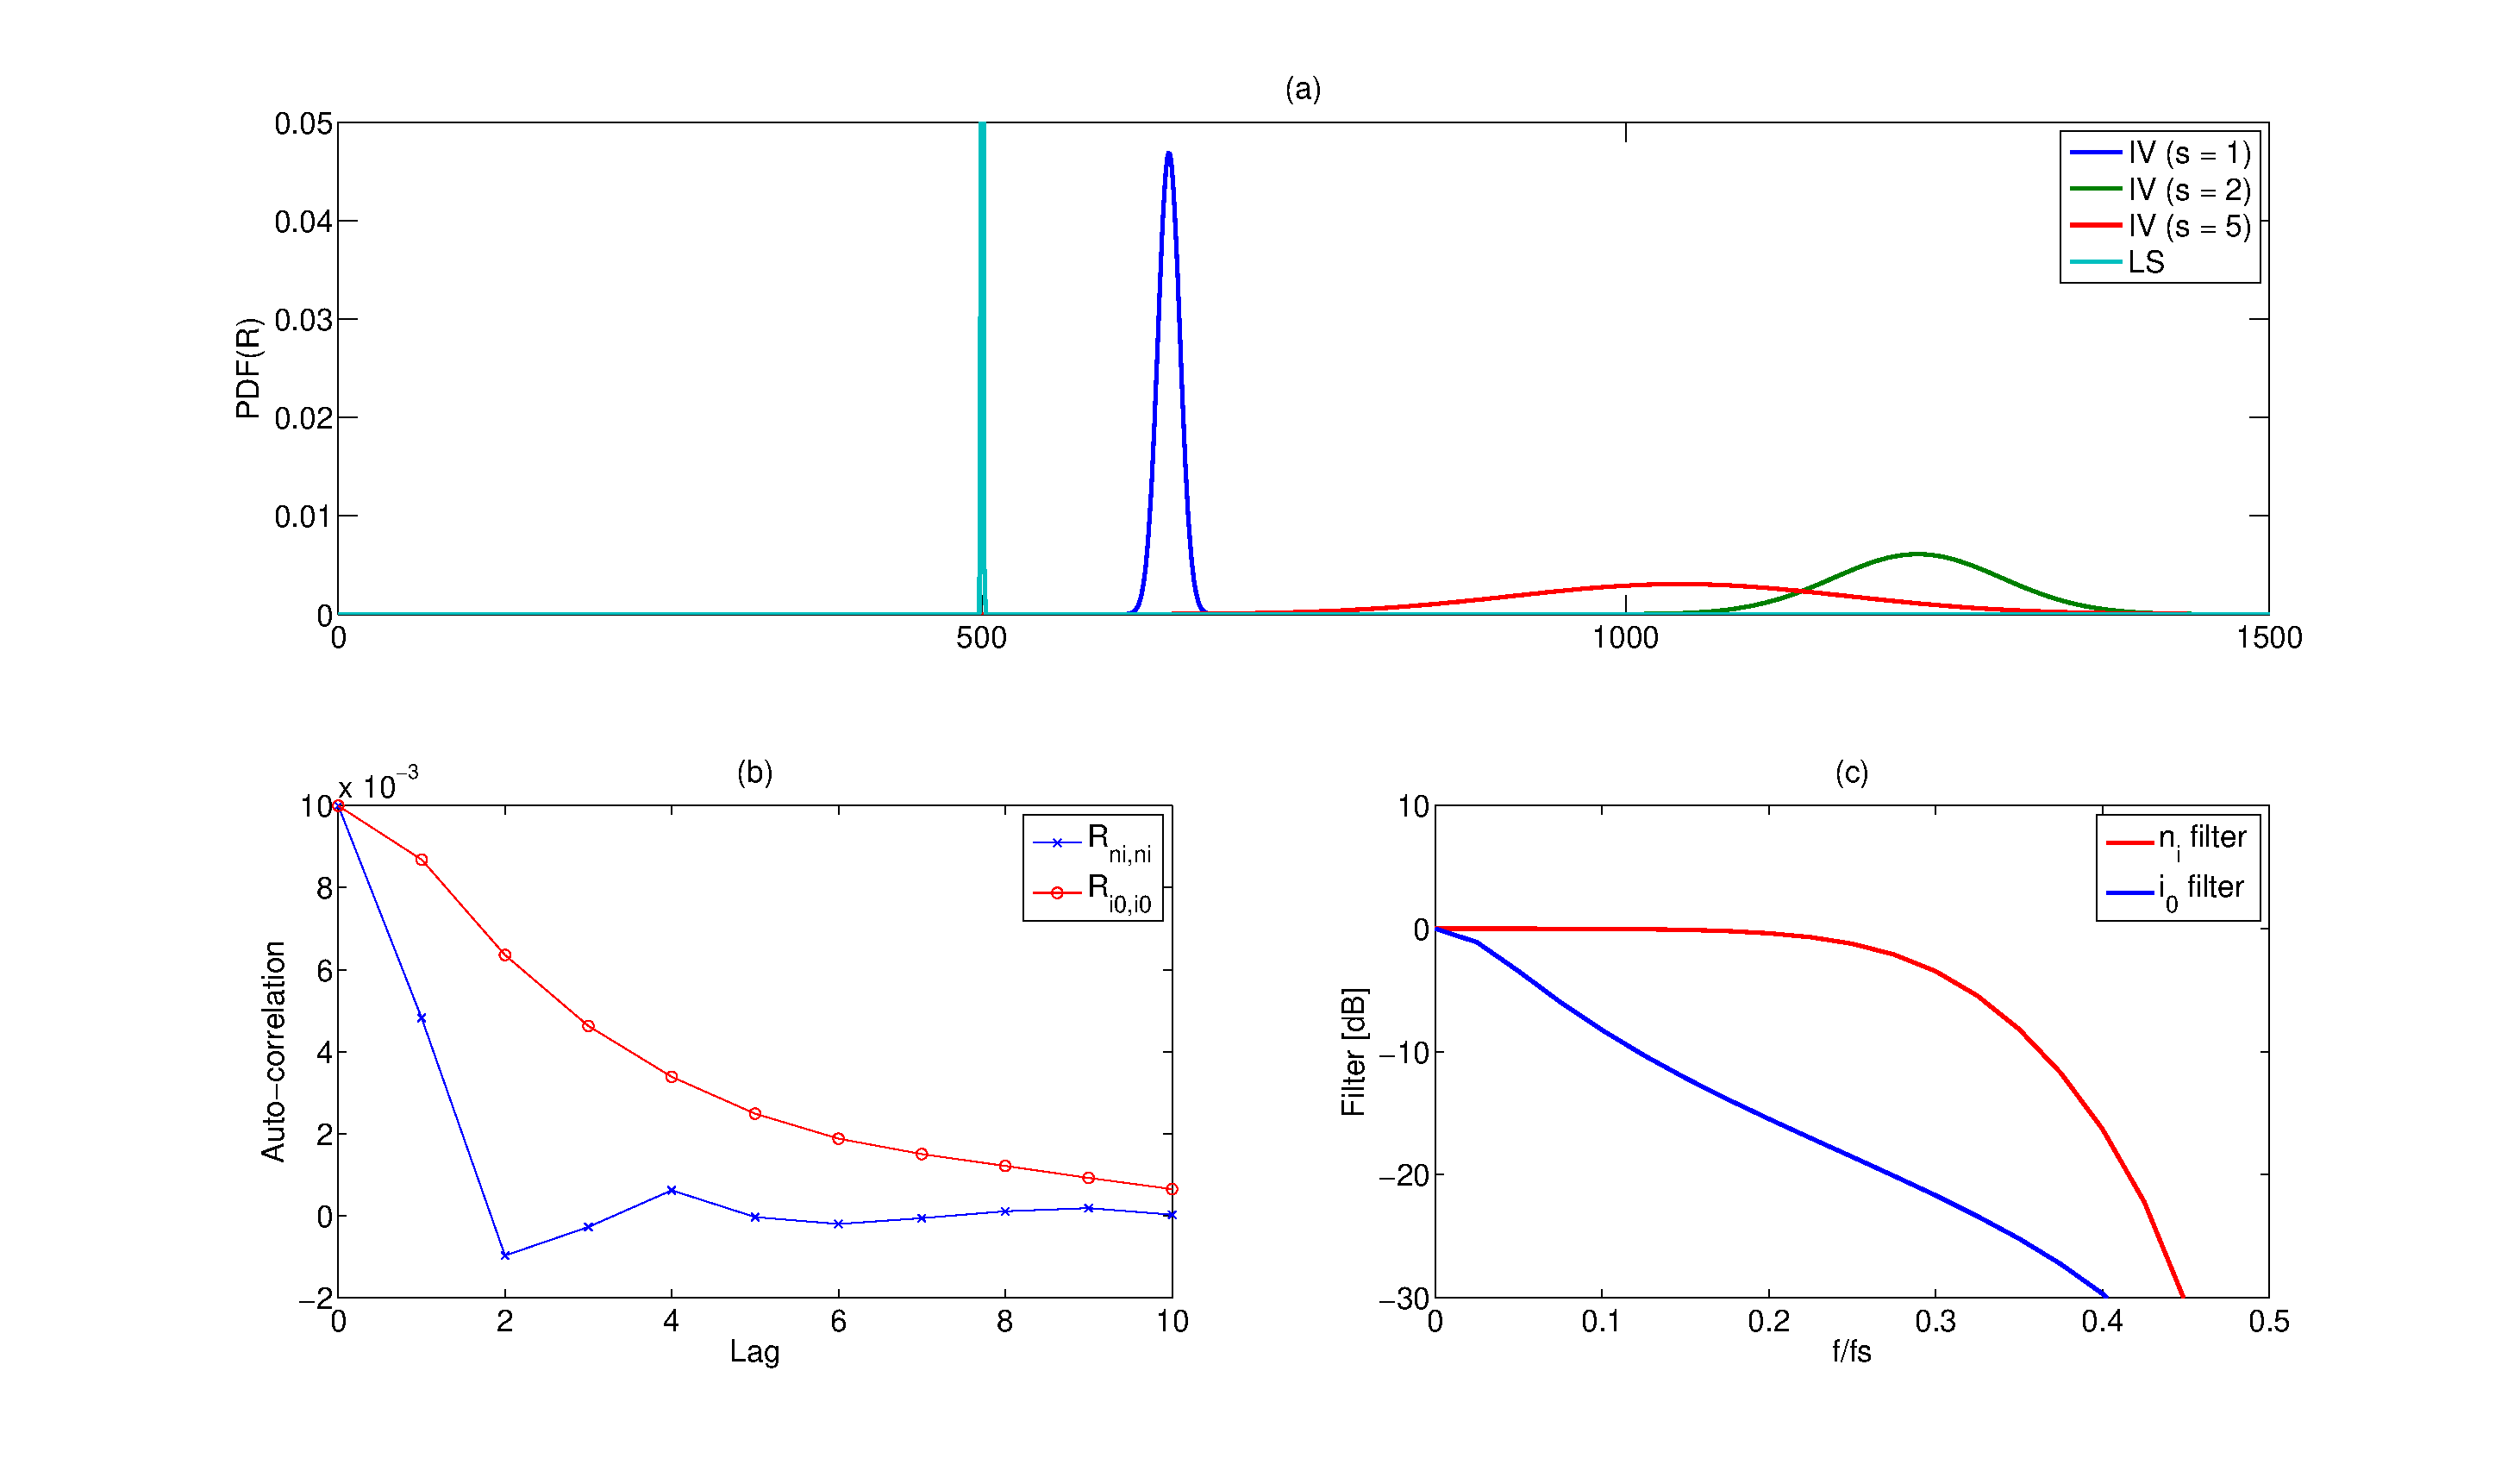
\includegraphics[width=1\textwidth]{figures/Sess1_part1_exp2.eps}
    \caption{Study of the LS and IV estimates for a fixed noise filter bandwidth and varying shift parameter $s =$ {1, 2, 5}. Fig. (a) : the LS (cyan) and IV estimates. IV(1) (blue), IV(2) (green) and IV(3) (red) correspond to a shift of 1, 2 and 5 respectively. Fig. (b): the auto-correlation of $i_0$ (red) and $n_i$ (blue). Fig. (c) : filter characteristics of $i_0$ (blue) and of $n_i$ (red).}
    \label{fig: Sess1_part1_exp2}
\end{figure}

\section{Experiment 3 : The errors-in-variables method}
For the first experiment, we use the following parameter settings : 

\begin{table}[h]
\centering
\begin{tabular}{ll}
    $ R_0 = 1000, $  &  $ sigma_{n_i} = 0.001, $   \\
    $ \sigma_{i_0} = 0.01, $  &  $ \sigma_{n_u} = 1, $   \\
\end{tabular}
\end{table}
The result of the first experiment are displayed on the figure~\ref{Sess1_part1_exp1}.

\paragraph{LS estimator} As can be seen on the top picture of fig.~\ref{Sess1_part1_exp1}, the LS estimate is biased. This bias is due to the fact that, with the LS estimate, we assume that the measured input is exact, which is not the case here because of the noise $n_i$. The relative bias is 1\% which is not large but still a bias.

TODO: try to express this as a function of the given parameter settings

\paragraph{EIV estimator} The EIV estimator has a mean of about 1000.1. Which means it has a bias of about 0.1\%. This bias will vanish if we increase the amount of experiments.

TODO: would the IV estimator work here?

\begin{figure}[H]
    \centering
    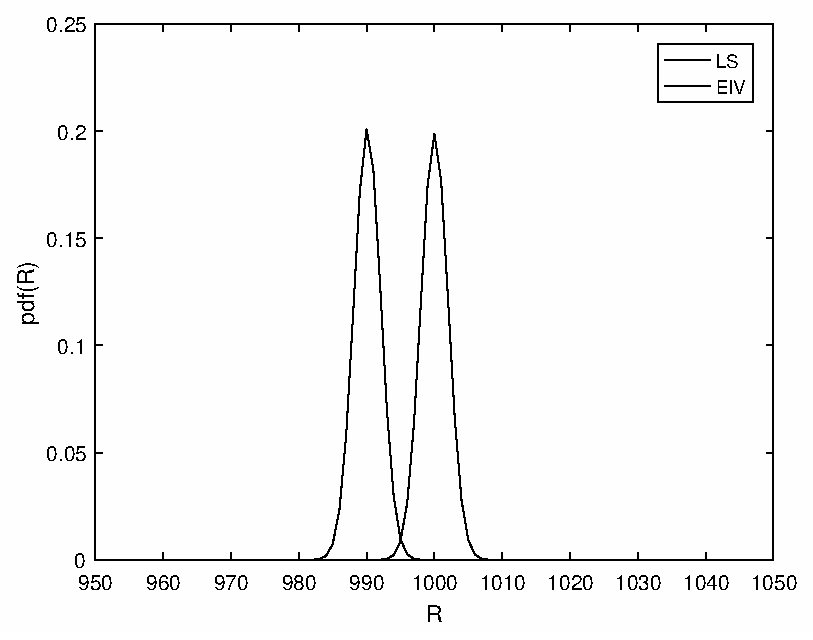
\includegraphics[width=1\textwidth]{Figures/Sess1_part2.eps}
    \caption{Comparison of the PDF of the LS and EIV estimate, calculated with prior known variables}
    \label{Sess1_part1_exp1}
\end{figure}



\appendix
% \section*{Codes}
% \addcontentsline{toc}{section}{Codes}
% \input{appendix/code.tex}

\end{document}




